\section{Conclusiones}

Para concluir, el diseño e implementación de la infraestructura de red para esta
empresa multinacional ha sido un proyecto desafiante pero sumamente
gratificante. Hemos logrado conceptualizar y poner en práctica una solución
robusta y escalable que no solo satisface las necesidades actuales de la
empresa, sino que también está preparada para adaptarse a su crecimiento futuro.
\\

La implementación de la topología de red en estrella ha proporcionado una
estructura confiable y eficiente para la gestión del tráfico de red. Al conectar
todas las sedes a un nodo central, hemos asegurado una comunicación fluida entre
todas las localidades, y la flexibilidad inherente a esta arquitectura nos
permitirá expandir y adaptar la red a medida que la empresa continúe creciendo.

\begin{figure}[H]
    \centering
    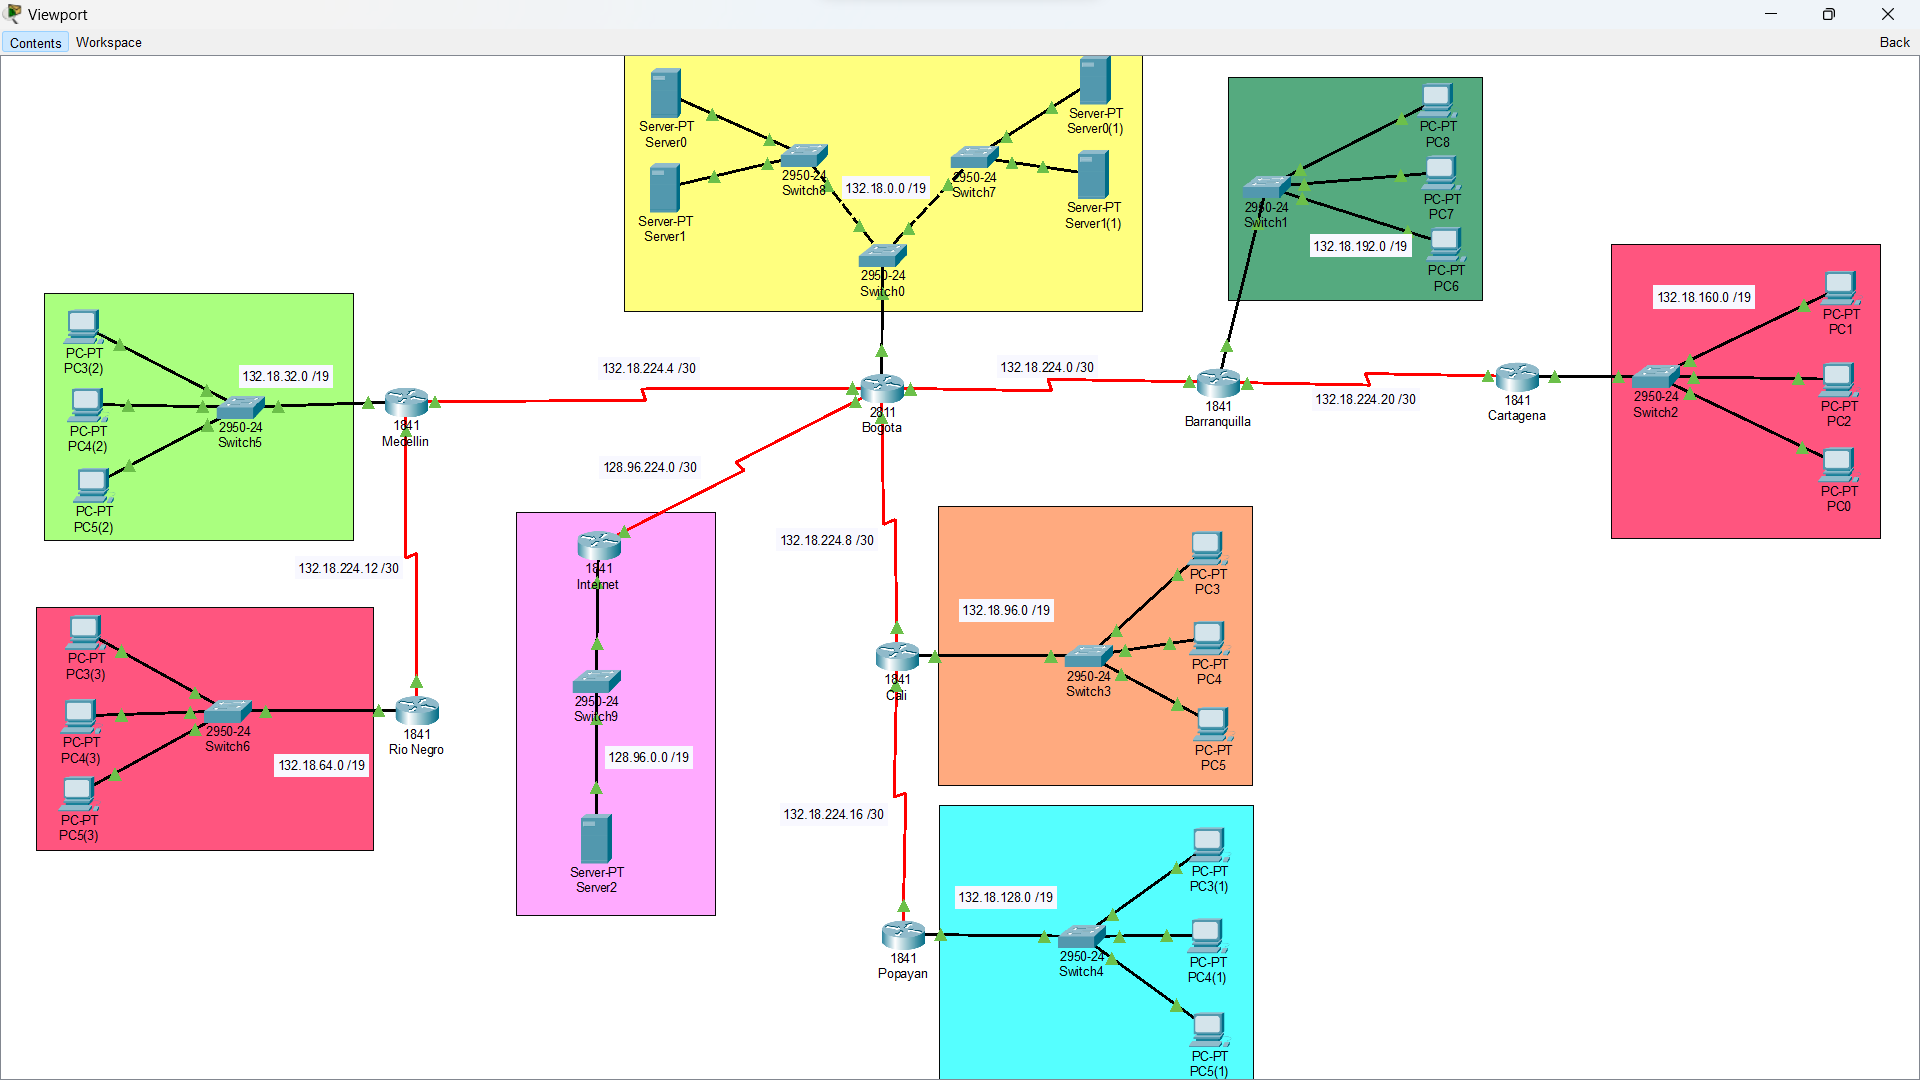
\includegraphics[width=0.7\textwidth]{Figures/4. Conclusions/final_result.png}
    \caption{Topología Completa de la red}
    \label{fig: Topologia Completa de la red}
\end{figure}

Además, el despliegue de la página web de la empresa en un clúster de servidores
web ha permitido manejar eficazmente un alto volumen de tráfico, garantizando un
rendimiento óptimo y una alta disponibilidad del sitio web. Esta solución ofrece
una gran tolerancia a fallos y permite ajustar los recursos de acuerdo con la
demanda, asegurando que la empresa pueda mantenerse al día con las necesidades
cambiantes de sus clientes.

\begin{figure}[H]
    \centering
    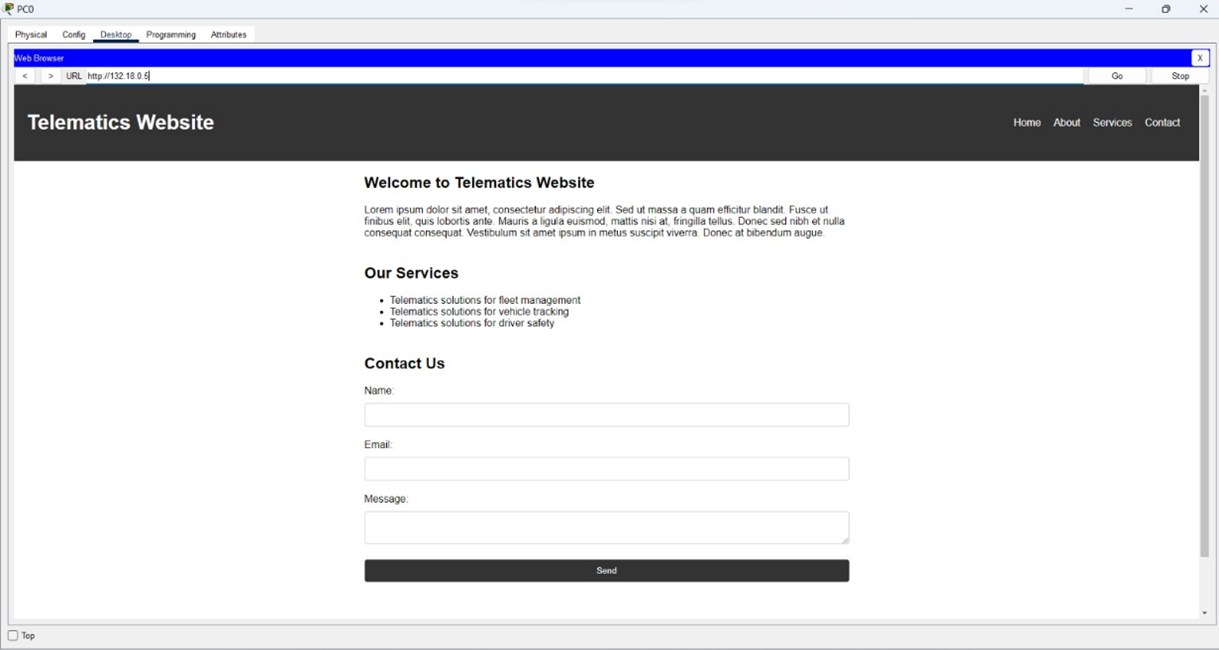
\includegraphics[width=0.7\textwidth]{Figures/4. Conclusions/web_page.png}
    \caption{Página web desplegada}
    \label{fig: deployed web page}
\end{figure}

\begin{figure}[H]
    \centering
    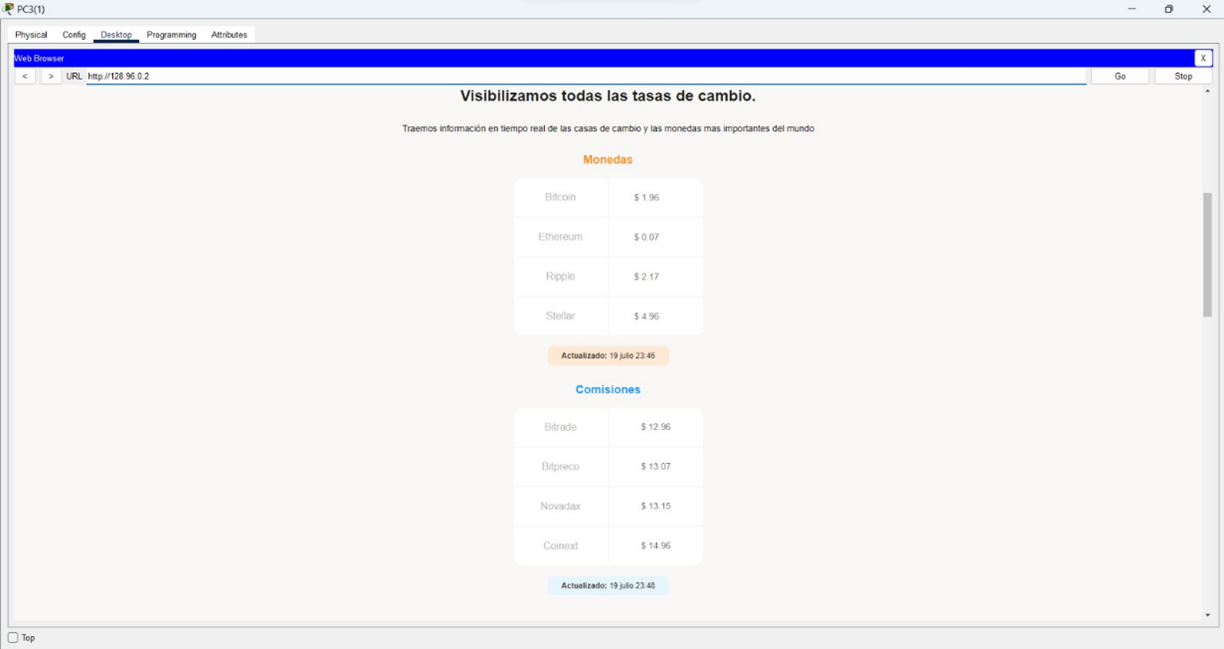
\includegraphics[width=0.7\textwidth]{Figures/4. Conclusions/internet_simulation.png}
    \caption{Simulación de acceso a internet}
    \label{fig: internet simulation}
\end{figure}

Además, la implementación de VLSM ha sido esencial para maximizar el uso del
espacio de direcciones IP y mejorar el rendimiento y la seguridad de la red. Al
permitir una asignación más eficiente del espacio de direcciones y políticas de
seguridad más granulares, VLSM ha demostrado ser una herramienta poderosa para
la gestión de redes.
\\

En una sección crucial de este proyecto, implementamos el Protocolo de Estado de
Enlace Abierto (Open Shortest Path First, OSPF) como nuestro protocolo de
enrutamiento dinámico. OSPF es un protocolo de enrutamiento de estado de enlace
que es ampliamente utilizado en redes de gran escala debido a su eficiencia,
escalabilidad y capacidad para recuperarse rápidamente ante fallos de red.
\\

La adopción de OSPF en nuestra infraestructura de red presenta varias ventajas
significativas. En primer lugar, OSPF es un protocolo de enrutamiento sin clase,
lo que significa que es compatible con VLSM y CIDR, permitiéndonos aprovechar
al máximo el espacio de direcciones IP disponible y mejorar la eficiencia de la
red.
\\

En segundo lugar, OSPF utiliza el algoritmo de Dijkstra para calcular la ruta
más corta a través de una red, lo que resulta en una gestión de tráfico
eficiente y efectiva. Este enfoque también garantiza una rápida convergencia de
la red en caso de fallos o cambios en la topología de la red, ya que cualquier
cambio en la topología se propaga rápidamente a través de la red.
\\

Además, OSPF admite el equilibrio de carga en múltiples rutas de igual costo, lo
que puede aumentar la disponibilidad y redundancia de la red. Esto es
especialmente útil en nuestra implementación, ya que nos permite manejar grandes
volúmenes de tráfico web de manera eficiente.
\\

Finalmente, OSPF es un protocolo de enrutamiento de código abierto, lo que
significa que no estamos atados a un proveedor específico de hardware de red y
tenemos una gran flexibilidad para adaptar y ajustar la configuración de la red
a nuestras necesidades específicas.
\\

Por lo tanto, la implementación de OSPF ha sido un componente clave para
asegurar una red robusta, resiliente y eficiente.
\\

En resumen, este proyecto ha sido un ejemplo de cómo un diseño de red cuidadoso
y una implementación eficaz pueden ayudar a una empresa a satisfacer sus
necesidades de conectividad, mejorar su rendimiento y asegurar su futuro
crecimiento. Estamos orgullosos de lo que hemos logrado y confiamos en que esta
infraestructura de red servirá bien a la empresa (del ejercicio) en los años 
venideros.